\let\negmedspace\undefined
\let\negthickspace\undefined
\documentclass[journal]{IEEEtran}
\usepackage[a5paper, margin=10mm, onecolumn]{geometry}
%\usepackage{lmodern} % Ensure lmodern is loaded for pdflatex
\usepackage{tfrupee} % Include tfrupee package

\setlength{\headheight}{1cm} % Set the height of the header box
\setlength{\headsep}{0mm}     % Set the distance between the header box and the top of the text

\usepackage{gvv-book}
\usepackage{gvv}
\usepackage{cite}
\usepackage{amsmath,amssymb,amsfonts,amsthm}
\usepackage{algorithmic}
\usepackage{graphicx}
\usepackage{textcomp}
\usepackage{xcolor}
\usepackage{txfonts}
\usepackage{listings}
\usepackage{enumitem}
\usepackage{mathtools}
\usepackage{gensymb}
\usepackage{comment}
\usepackage[breaklinks=true]{hyperref}
\usepackage{tkz-euclide} 
\usepackage{listings}
% \usepackage{gvv}                                        
\def\inputGnumericTable{}                                 
\usepackage[latin1]{inputenc}                                
\usepackage{color}                                            
\usepackage{array}                                            
\usepackage{longtable}                                       
\usepackage{calc}  
\usepackage{amsmath,amssymb}

\usepackage{multicol}                                         
\usepackage{hhline}                                           
\usepackage{ifthen}                                           
\usepackage{lscape}
\begin{document}

\bibliographystyle{IEEEtran}

\title{
%	\logo{
NCERT - 12.6.5.28

\large{EE1003}
%	}
}
\author{Homa Harshitha Vuddanti

(EE24BTECH11062)
}	

\maketitle

\bigskip

\renewcommand{\thefigure}{\theenumi}
\renewcommand{\thetable}{\theenumi}
\textbf{Question}: For all real values of $x$ find the minimum and maximum value of $\frac{1-x+x^2}{1+x+x^2}$.\\
\textbf{Theoretical solution: }\\
Given,
\begin{align}
f\brak{x}=\frac{1-x+x^2}{1+x+x^2}
\end{align}
For finding the values, we first find the critical points where $f^\prime\brak{x}=0$. 
\begin{align}
f^\prime\brak{x}&=
\frac{\brak{2x-1}\brak{1+x+x^2}-\brak{2x+1}\brak{1-x+x^2}}{\brak{1+x+x^2}^2}\\
f^\prime\brak{x}&=\frac{2\brak{x^2-1}}{\brak{1+x+x^2}^2}=0
\end{align}
Solving, we get $x=1$ and $x=-1$. To find the minimum and maximum, we do the second derivative test.
\begin{align}
f^{\prime\prime}\brak{x}=\frac{\brak{4x}\brak{1+x+x^2}^2-4\brak{x^2-1}\brak{1+x+x^2}\brak{2x+1}}{\brak{1+x+x^2}^4}\\
\end{align}
$f^{\prime\prime}\brak{1}>0$, so it is the minimum, while $f^{\prime\prime}\brak{-1}<0$ so it is the maximum.
Therefore, the minimum value is $f\brak{1}=\frac{1}{3}$, which occurs at $x=1$ and the maximum value is $f\brak{-1}=3$.\\
\textbf{Gradient Descent method :}\\
We can use the gradient descent method to find the minimum of our curve. The algorithm iterates as follows:
\begin{align}
x_{n+1}=x_n-\alpha f^\prime\brak{x}
\end{align}
Here, $\alpha$ controls the step size and we stop when the difference between $x_{n+1}$ and $x_n$ becomes very small beyond a convergence threshold.
\begin{align}
x_{n+1}=x_n-\alpha\brak{\frac{2\brak{x_n^2-1}}{\brak{1+x_n+x_n^2}^2}}
\end{align}
\textbf{Gradient ascent method:} We can find the maximum value of the function using gradient ascent method.
\begin{align}
x_{n+1}=x_n+\alpha f^\prime\brak{x}\\
x_{n+1}=x_n+\alpha\brak{\frac{2\brak{x_n^2-1}}{\brak{1+x_n+x_n^2}^2}}
\end{align}
\textbf{Plotting:}\\
Taking 
\begin{align}
x_0=0.5\\
\alpha=0.01\\
threshold=10^{-6}\\
n=1000
\end{align}
\begin{figure}[h!]
   \centering
   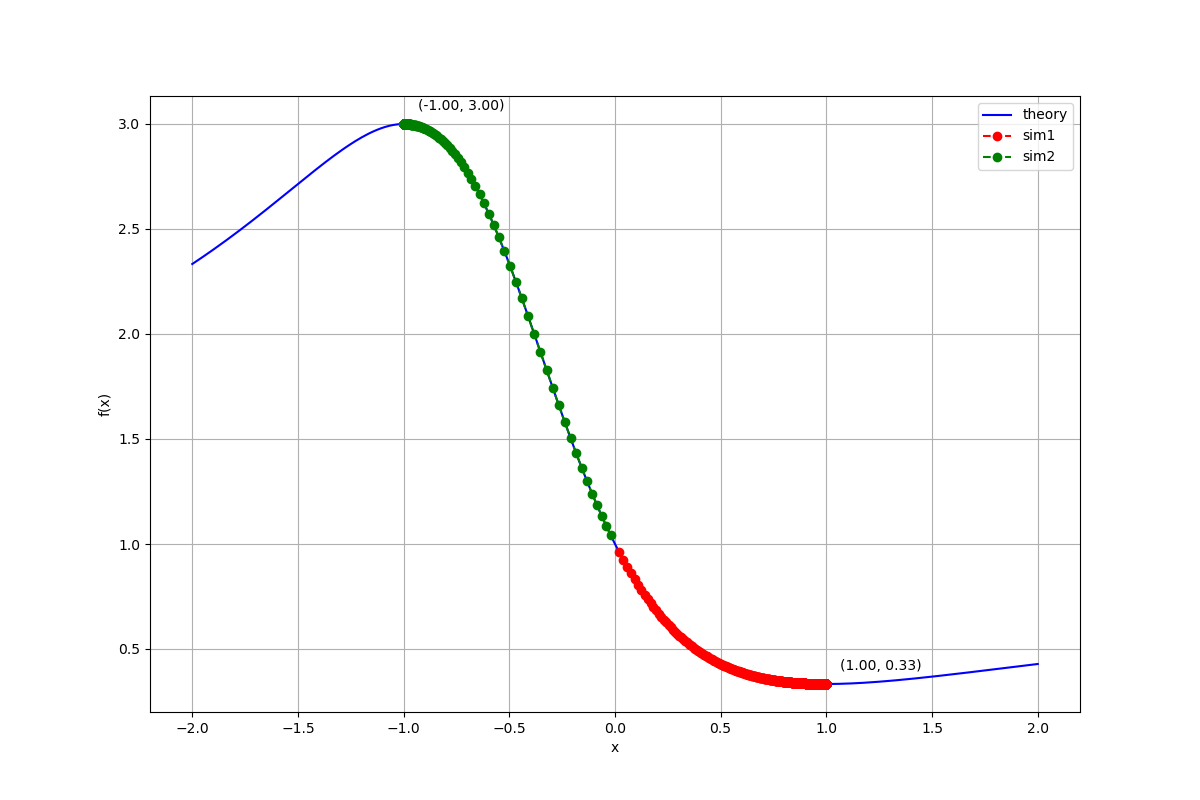
\includegraphics[width=1\columnwidth]{Figs/Figure_1.png}
   \caption{Plot}
\end{figure}
\end{document}



